\def \sectionauthors {Samuel Bleiner}
\subsection{Anforderungen}
\lipsum[1-5]
\subsection{Vorstudie}
\lipsum[1-5]

\subsection{Bildverarbeitung}

\subsubsection{Einleitung}
Die Bildverarbeitung ist ein zentrales Thema in dieser Applikation für Kennzeichenerkennung. 
Sie wird für die Zeichensegmentierung verwendet, sowie für die Vorbereitung von Bildern für 
andere Algorithmen. Im Folgenden werden die verwendeten Bildverarbeitungsfunktionen aufgelistet 
und deren Funktionsweise erläutert.

\subsubsection{Bilaterale Filterung}
Bilaterale Filterung ist eine Methode für eine kantenerhaltende Weichzeichnung eines Bildes.\\

Bei der Berechnung für den Farbwert des Ausgabepixels werden die benachbarten Pixel nicht nur 
mit ihrer Entfernung gewichtet, sondern auch mit ihrem eigenen Farbwert. Dadurch können einzelne 
farbliche Ausreißer herausgefiltert werden. Dies ist vor allem in der Bildverarbeitung wichtig, 
da dadurch die wichtigen Eigenschaften eines Bildes, wie zum Beispiel Kanten, erhalten bleiben 
und verarbeitet werden können, aber einzelne abweichende Pixel herausgefiltert werden wodurch 
unnötige Informationen entfernt werden.\\ 

In Abbildung 1 kann man ein Bild von verschieden Lebensmitteln sehen. Wenn man genau hinsieht 
erkennt man vor allem bei den Blättern im Hintergrund und beim Brot viele detailreiche Texturen. 
Diese Texturen haben keine wichtige Texturen und sind deswegen unnötig. Um die Bildverarbeitung zu 
vereinfachen wendet man deswegen die bilaterale Filterung auf dieses Bild an, um diese detailreichen 
Texturen zu vereinfachen. In Abbildung 2 sieht man das Bild nach der bilateralen Filterung. 
Wenn man hier dann wieder genauer auf die Blätter und das Brot sieht, erkennt man, dass die 
detailreichen Texturen weichgezeichnet wurden, aber die Kanten sind genauso gut erkennbar wie vor der Filterung.

\subsubsection{Thresholding}
Das Thresholding oder auch Schwellenwertverfahren wird in der Bildverarbeitung verwendet, um Bilder zu segmentieren. 
Aus einem Graubild kann dadurch ein Binäres Bild erzeugt werden.\\ 

Bei diesem Verfahren wird ein bestimmter Schwellwert (En.: Threshold) definiert, welcher mit den Grauwerten der einzelnen 
Pixel des Bildes verglichen wird. Wenn der Grauwert den Schwellwert überschreitet, wird dieser durch einen weißen Pixel 
ersetzt und wenn der Grauwert kleiner als der Schwellwert ist, wird dieser durch einen schwarzen Pixel ersetzt. 
Dadurch erhält man ein Bild welches nur noch zwei Farben hat, Schwarz und Weiß. Dies wird deswegen eingesetzt, 
da dadurch viele Bildverarbeitungsalgorithmen schneller arbeiten und die Effizienz gesteigert wird.\\

In Abbildung 3 sieht man ein solches Graubild welches nur verschieden Graustufen aufweist. In Abbildung 4 sieht man das 
Bild nach dem Thresholding. Hier kann man nur noch das Boot mit den Menschen erkennen. Dies ist nicht nur für schnellere 
Bildverarbeitungsalgorithmen wichtig, sondern wird auch zur Objekterkennung in Bildern verwendet.\\

Um den Schwellwert zu bestimmen kann man diesen entweder variieren bis das gewünschte Ergebnis erscheint oder man 
verwendet Methoden, welche den Schwellwert automatisch bestimmen. Eine der bekanntesten Methoden zur Schwellwertbestimmung 
ist die Methode von Otsu, welche mit dem Schwellenwert die Pixel in Vordergrund und Hintergrund unterteilt.

\subsubsection{Erosion}
Erosion ist eine Funktion der Bildverarbeitung und ist in die morphologische Bildverarbeitung einzuordnen. Diese beschäftigt 
sich primär mit der Verarbeitung von binären Bildern, welche man nach Thresholding erhält.\\

Erosion benötigt zwei Eingaben, das binäre Bild und einen Kernel. Der Kernel ist dabei die Angabe, nach welcher die Erosion 
durchgeführt wird. Der Kernel ist auch eine binäre Struktur, welche über jeden einzelnen Pixel des binären Bildes geschoben 
wird. Wenn der Kernel komplett mit dem binären Bild übereinstimmt, behält dieser Pixel seinen Wert und ansonsten wird er 
invertiert. Dabei muss jedoch darauf geachtet werden, dass die Polarität des binären Bildes und des Kernels übereinstimmt, 
da sonst die Erosion nicht richtig funktioniert. Als Resultat erhält man danach ein deutlicheres Bild bei welchem einzelne 
Pixelfehler herausgefiltert wurden und die Konturen besser erkennbar sind.\\

In Abbildung 5 und 6 sieht man die Anwendung der Erosion. Die Konturen der einzelnen Zeichen im Kennzeichen sind in Abbildung 
6 nach der Erosion deutlicher erkennbar als davor.

\subsubsection{Farbraum}
Der Farbraum eines Bildes enthält alle möglichen Farben eines Farbmodells. Das Farbmodell beschreibt dabei die Parameter, aus 
welchen die einzelnen Farben gebildet werden. Dies ist in der Bildverarbeitung relevant, da verschiedene Funktionen der 
Bildverarbeitung, unterschiedliche Farbräume verwenden und dieser deswegen korrekt eingestellt werden muss.\\

In dieser spezifischen Applikation werden die folgenden Farbräume verwendet:

\paragraph{RGB}\mbox{}\\
RGB ist einer der häufigsten und bekanntesten Farbräume. Er basiert auf den drei Grundfarben Rot, Grün und Blau und wird vor 
allem bei Bildschirmen und in der Fotografie genutzt. Die Farben setzen sich in diesem Modell aus dem jeweiligen Rot-, Grün- 
und Blauanteil der einzelnen Pixel zusammen.

\paragraph{Graustufen}\mbox{}\\
Bei einem Graustufen-Bild, zu sehen in Abbildung 3, hat jeder Pixel einen Wert von 0 bis 255. Diese Werte erstrecken sich also 
von Schwarz bis Weiß und dazwischen liegen verschiedene Grautöne. Dieser Farbraum wird in der Bildverarbeitung häufig verwendet, 
da Konturen einfacher erkennbar sind und es nur einen Parameter gibt, welcher verarbeitet werden muss, wodurch die Effizienz 
diverser Algorithmen gesteigert werden kann. Zudem wird dieser Farbraum auch oft in Verbindung mit Thresholding verwendet.

\paragraph{BGR}\mbox{}\\
Der BGR ist ein relativ unbekannter und wenig verwendeter Farbraum, da er sehr ähnlich zum RGB-Farbraum ist. Der einzige 
Unterschied zwischen diesen beiden liegt in der Anordnung der Parameter. Bei BGR sind die Parameter spiegelverkehrt zu RGB, 
das heißt es kommt zuerst der Blauanteil, dann der Grünanteil und zum Schluss der Rotanteil. Insgesamt ergibt dies für die 
einzelnen Pixel zwar die gleichen Farben, aber die Funktionen der Bildverarbeitung müssen trotzdem das Bild im passenden 
Farbraum erhalten. So verwendet zum Beispiel die Funktion „imread“ von OpenCV den BGR-Farbraum und die Funktion „im Show“ 
von Matplotlib verwendet den RGB-Farbraum. Wenn man diese Funktionen also nacheinander anwendet, muss dazwischen der Farbraum 
umgewandelt werden.

\subsubsection{Konturerkennung}
Die Konturerkennung ist eine wichtige Funktion in der Bildverarbeitung mit welcher Objekte in einem Bild gefunden werden können. 
In dieser Applikation wird sie für die Zeichensegmentierung eingesetzt.\\

Die Konturerkennung wird hauptsächlich bei binären Bildern verwendet. Eine Kontur kann dabei wie im Folgenden definiert werden. 
Man überprüft jeden einzelnen Pixel und sieht nach, ob ein benachbarter Pixel einen anderen Farbwert aufweist. Falls dies 
zutrifft muss der zu prüfende Pixel zu einer Kontur gehören. Wenn dies auf mehrere zusammenhängende Pixel zutrifft, bedeutet 
das, dass diese zusammen eine Kontur bilden.\\

Die Funktion „findcontours“ von OpenCV, welche in dieser Applikation verwendet wird, ist eine Funktion für Konturerkennung 
und kann weiße Objekte auf einem schwarzen Hintergrund erkennen. Sie basiert auf dem Algorithmus von Suzuki von 1985 und 
liefert eine Liste mit allen Konturen. Die Konturen werden in der Liste als ein Array von Koordinaten abgespeichert.

\subsection{Kennzeichenerkennungsprogramm}

\subsubsection{Einleitung}
Die Software ist der wichtigste und größte Teil der Kennzeichenerkennung. Sie erhält ein Bild, in welchem ein Auto mit 
einem Kennzeichen enthalten ist und liefert am Ende dieses Kennzeichen und sendet dieses dann automatisch an die Datenbank. 
Die Software kann entweder über Bildverarbeitung oder mit Machine Learning Modellen realisiert werden. Der erste Ansatz bei 
dieser Anwendung war mit klassischer Bildverarbeitung, welche aber nicht die gewünschte Genauigkeit erreicht hat, weswegen 
dann auf Machine Learning gewechselt wurde.

\subsubsection{Programmiersprache}
Die verwendete Programmiersprache für die Kennzeichenerkennung ist Python. Python ist eine höhere Programmiersprache, 
welche übersichtlich und leicht lesbar ist. Sie ist vor allem für Bildverarbeitung und Machine Learning Anwendungen gut geeignet, 
da es dafür hoch optimierte und effiziente Bibliotheken gibt wie zum Beispiel OpenCV, Numpy und Tensorflow. Dadurch ist Python 
für diese Anwendung besser geeignet als zum Beispiel C++. Dieses wäre zwar normalerweise effizienter, bietet aber weniger 
optimierte Bibliotheken in diesem Bereich, wodurch es hier weniger gut geeignet ist.

\subsubsection{Konzept}
Das Programm für die Kennzeichenerkennung basiert auf fünf Stufen. Die erste Stufe ist die Bildaufnahme, die zweite ist die 
Kennzeichenerfassung mittels Machine Learning, die dritte ist die Kennzeichensegmentierung mithilfe von Bildverarbeitung, 
die vierte ist die Zeichenerkennung mittels Machine Learning und die fünfte ist die Anbindung an die Datenbank.

\paragraph{Bildaufnahme}\mbox{}\\
Um ein Bild verarbeiten zu können und aus diesem ein Kennzeichen auslesen zu können, muss zuerst ein Bild vorliegen. 
Dieses wird über den RaspberryPi mit der RaspberryPi-Kamera aufgenommen. Um das Bild aufzunehmen, muss einfach ein Auslöser 
aktiviert werden und dann wird das Bild aufgenommen und im richtigen Ordner abgespeichert. Zuvor wird noch überprüft ob 
sich in diesem Ordner bereits ein Bild befindet und falls eines vorhanden ist wird es gelöscht. Dadurch werden mögliche Fehler 
durch mehrere Bilder verhindert.

\paragraph{Kennzeichenerfassung}\mbox{}\\
Die Kennzeichenerfassung hat die Aufgabe, das Kennzeichen im Eingabebild zu lokalisieren. Dies geschieht mittels Machine Learning 
mit dem Modul WPOD-NET von Sérgio Montazolli Silva und Cláudio Rosita Jung. Dieses verwendet zuerst das Modul YOLOv2 welches zur 
Echtzeitobjekterkennung verwendet werden kann und in dieser Anwendung zur Erkennung von Fahrzeugen verwendet wird. Danach werden 
die Koordinaten des Kennzeichens ermittelt und dieses aus dem Bild ausgeschnitten und abgespeichert.

\paragraph{Kennzeichensegmentierung}\mbox{}\\
Die Kennzeichensegmentierung hat das Ziel die einzelnen Zeichen im Kennzeichen zu separieren und so zu vorbereiten, dass die 
darauffolgende Zeichenerkennung damit arbeiten kann. Dazu wird das Bild mit dem Kennzeichen zuerst in Graustufen konvertiert, 
dann mit einem bilateralen Filter gefiltert, mit Thresholding in ein binäres Bild umgewandelt und anschließend mittels Erosion 
besser erkennbar gemacht. Danach werden im verarbeiteten Bild die Konturen gesucht, sortiert und anhand dieser die einzelnen Zeichen herausgefiltert.

\paragraph{Zeichenerkennung}\mbox{}\\
Die letzte Stufe der Kennzeichenerkennung ist die Zeichenerkennung. In dieser werden die einzelnen Zeichen erkannt und als Text 
abgespeichert. Dies funktioniert über eine eigenes Neuronales Netz basierend auf MobileNetV2, welches mit einem Datensatz von 
über 35 000 Bildern auf die Erkennung von Zeichen aus Bildern trainiert wurde.

\paragraph{Anbindung an Datenbank}\mbox{}\\
Nachdem das Kennzeichen als Text abgespeichert wurde, muss diese Information in die Datenbank übergeben werden. Dazu wird die 
eigene API angewandt, welcher man diese Informationen übergeben muss und als Rückgabe die Information bekommt, ob sich das 
Fahrzeug nun innerhalb oder außerhalb des Parkplatzes befindet.

\paragraph{Ablauf}\mbox{}\\

\begin{figure}[H]
    \centering
    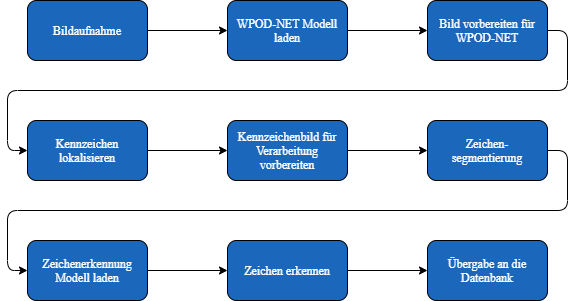
\includegraphics[width=0.9\linewidth]{kennzeichenerkennung/Programmablauf.png}
    \caption{Ablaufdiagramm der Kennzeichenerkennung}
\end{figure}

Im oberen Diagramm ist der Ablauf des Programms angegeben. Zuerst wird mit einem Button der Auslöser betätigt und damit das 
Foto aufgenommen. Dann wird das erste Machine Learning Modell für die Kennzeichenerkennung „WPOD-NET“ geladen. Bevor das 
Bild diesem Modell übergeben werden kann, muss es noch angepasst werden damit das Modell damit arbeiten kann. Danach kann 
damit das Kennzeichen im Bild lokalisiert werden. Im Anschluss wird dieses Kennzeichenbild mit mehreren Bildverarbeitungsalgorithmen 
verarbeitet, um dann die einzelnen Zeichen zu segmentieren. Danach kann dann das Modell für die Zeichenerkennung geladen 
werden und dieses dann auch angewendet werden, um das Ergebnis zu erhalten. Dieses Ergebnis wird dann noch mit einer API an die Datenbank übergeben.

\subsection{Raspberry Pi}

\subsubsection{Einleitung}
Damit die Software der Kennzeichenerkennung arbeiten kann, benötigt es eine geeignete Hardware. Diese muss dabei die folgenden Eigenschaften 
aufweisen, um für die Kennzeichenerkennung geeignet zu sein:

\begin{itemize}
    \item Möglichst klein
    \item Nicht zu teuer 
    \item Möglichkeit eine Kamera anzuschließen 
    \item Schnell 
    \item Internetanbindung
\end{itemize}

\subsubsection{Wahl des Raspberry Pi}
In dieser Applikation wird ein RaspberryPi 4B 2GB verwendet, da er alle zuvor genannten Eigenschaften am besten erfüllt.\\

\begin{figure}[H]
    \centering
    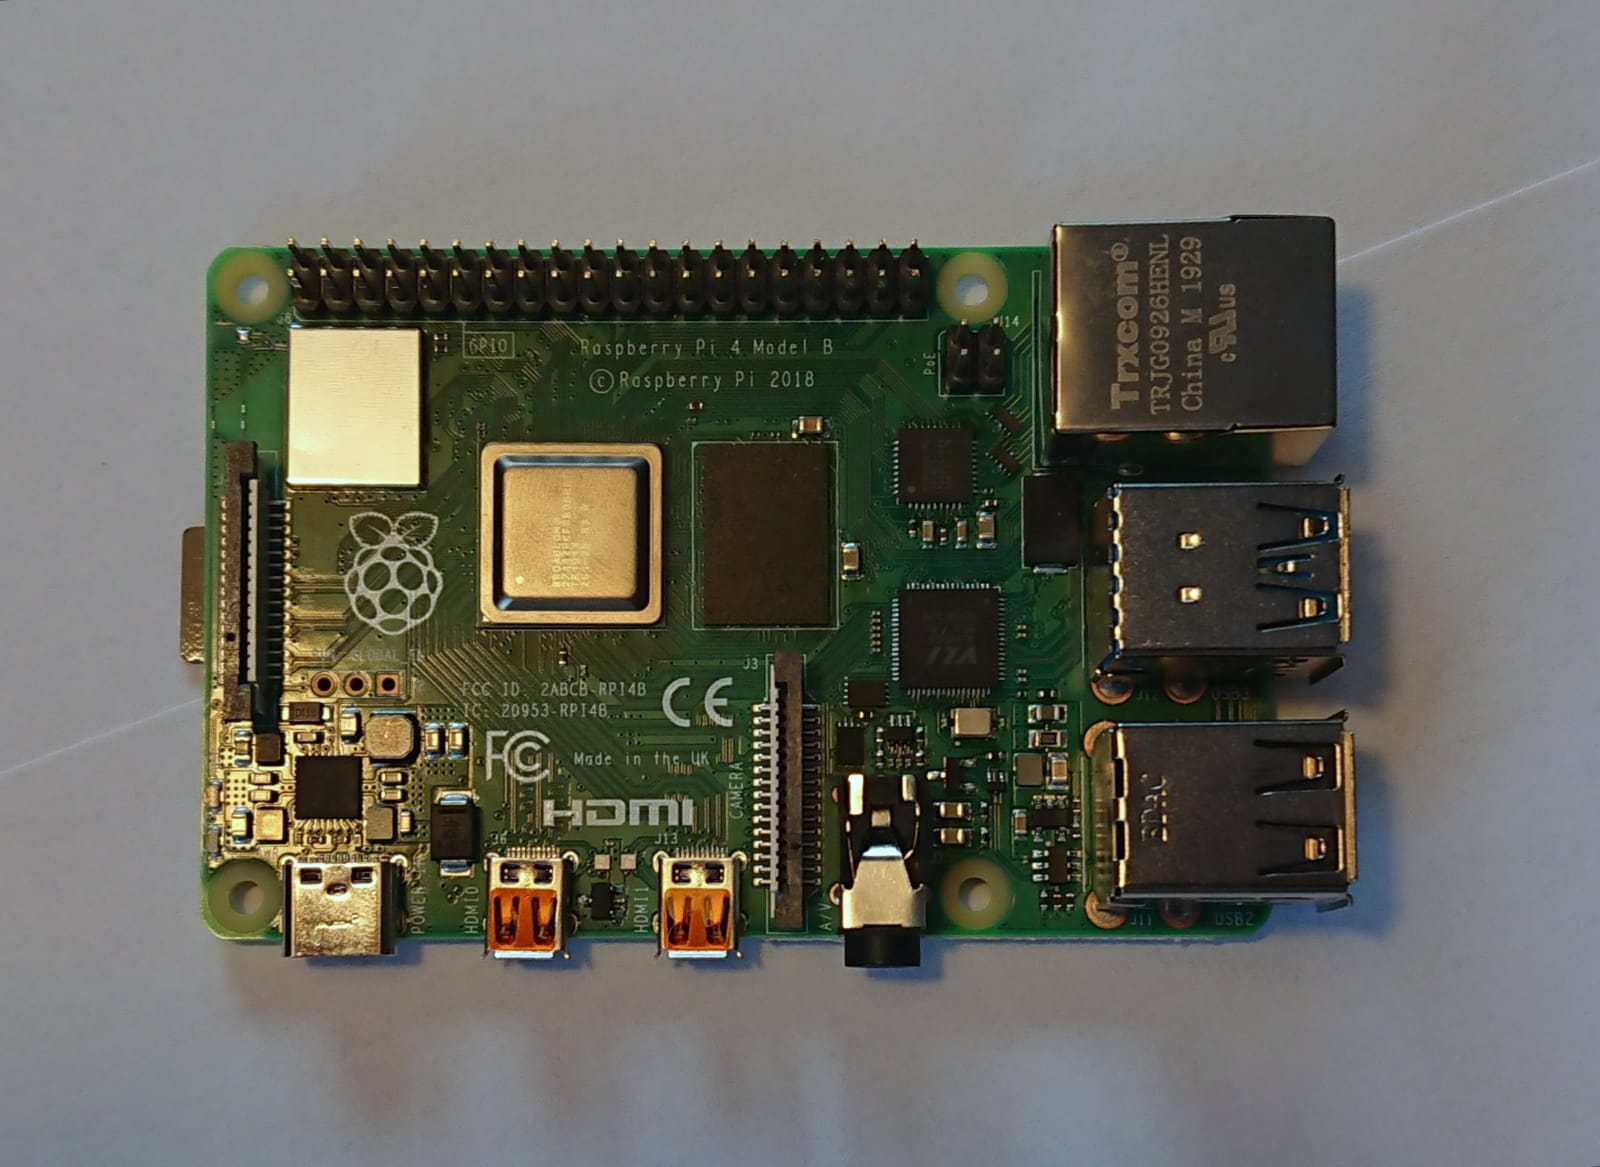
\includegraphics[width=0.6\linewidth]{kennzeichenerkennung/rpi.png}
    \caption{Raspberry Pi}
\end{figure}

Er hat die Größe einer Scheckkarte, wodurch es möglich ist ein kompaktes Gehäuse zu bauen, welches man einfach montieren kann. 
Er ist mit 35€ pro Stück nicht zu teuer. Er hat einen integrierten Kameraanschluss und es gibt unzählige Kameras, welche damit 
kompatibel sind. Er hat für seine Größe eine sehr gute Rechenkraft und ist damit in der Lage das komplette Programm für die 
Kennzeichenerkennung in einer akzeptablen Zeit abzuarbeiten. Er besitzt außerdem einen Ethernet-Anschluss und ein WLAN-Modul, 
wodurch er sehr einfach mit dem Internet verbunden werden kann.

\subsubsection{Kamera}
Für den Raspberry Pi muss zudem noch die passende Kamera ausgewählt werden, um die Bilder von den Kennzeichen aufzunehmen. 
Dafür gibt es Unmengen an kompatiblen Kameras, aber hier wird das Originalzubehör von RaspberryPi verwendet. Dies hat den Grund, 
dass diese Kamera leicht zu verwenden, sehr klein, mit Schrauben einfach zu befestigen und günstig ist. Zudem liefert sie ein 
qualitativ hochwertiges Bild, welches für die Software gut verarbeitbar ist.

\begin{figure}[H]
    \centering
    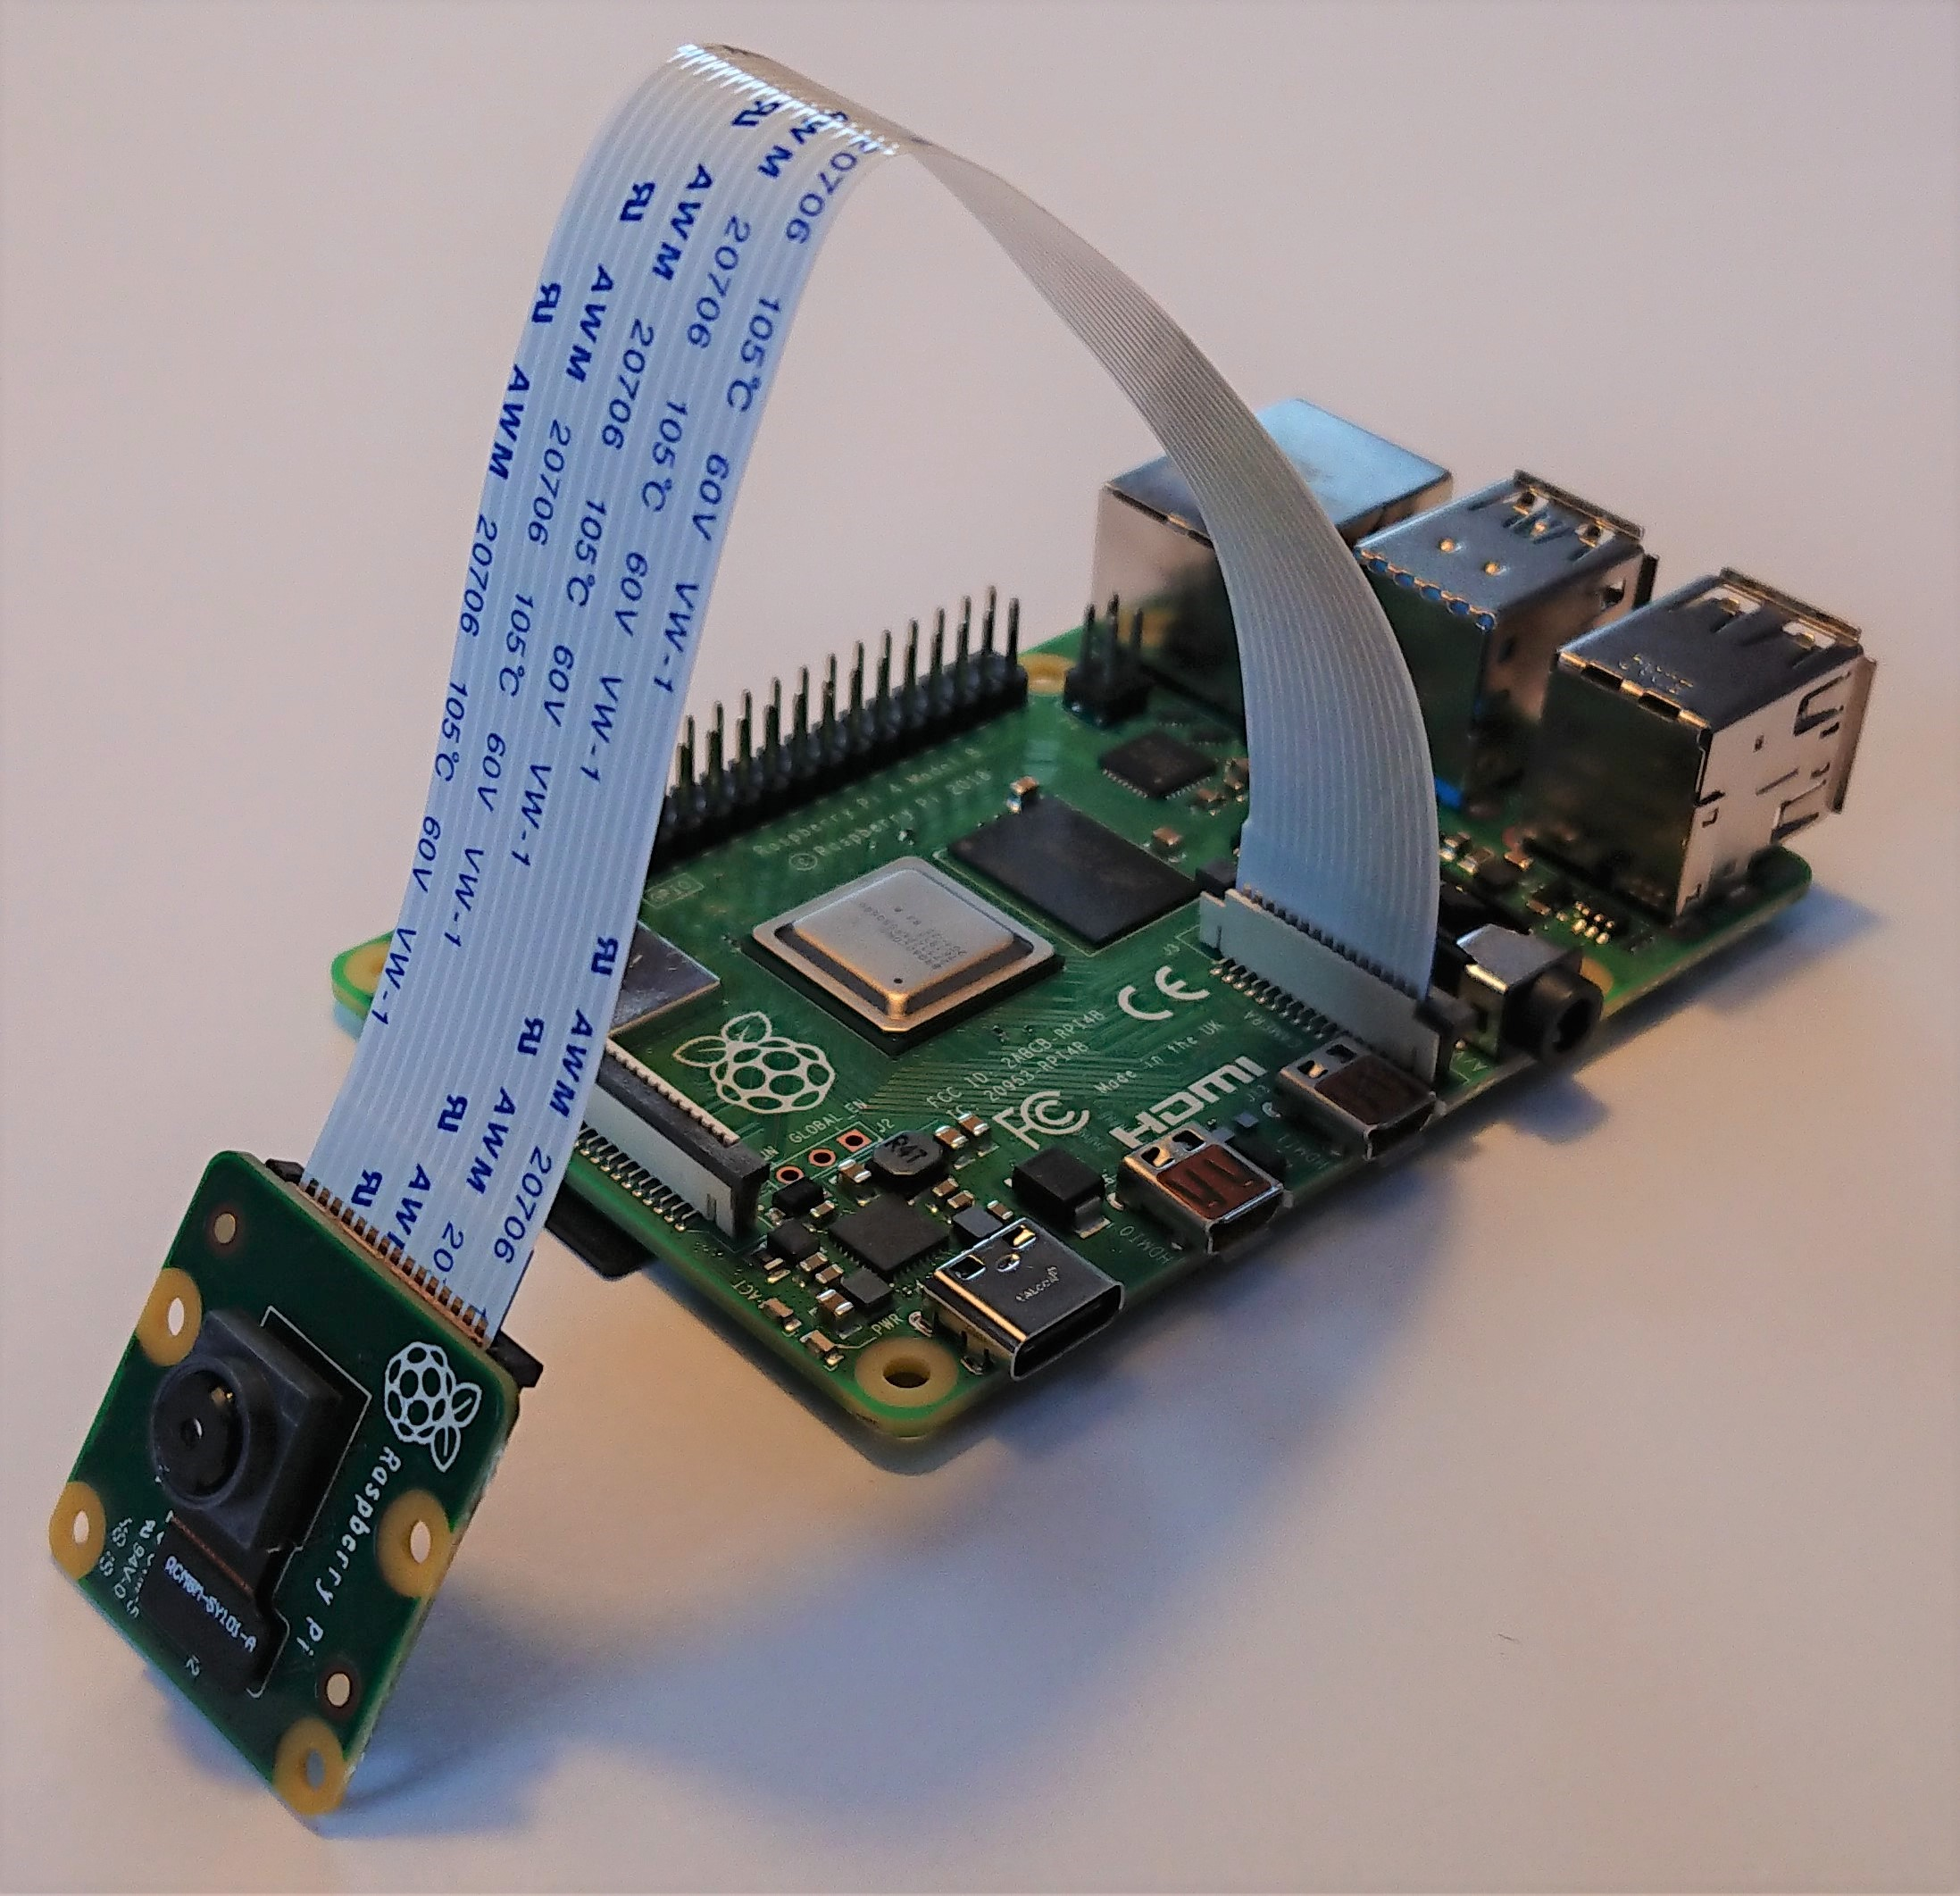
\includegraphics[width=0.6\linewidth]{kennzeichenerkennung/rpiKamera.png}
    \caption{Raspberry Pi mit Kamera}
\end{figure}